\section{ Test Scenarios and Study Region}

We tested the proposed method on four different idealized domains and a real heterogenous domain. The idealized domains are homogeneous and layered. Figure.~\ref{fig:3d_domain_scenarios}  represents these domains. 

 \begin{figure}[ht]
    \centering
    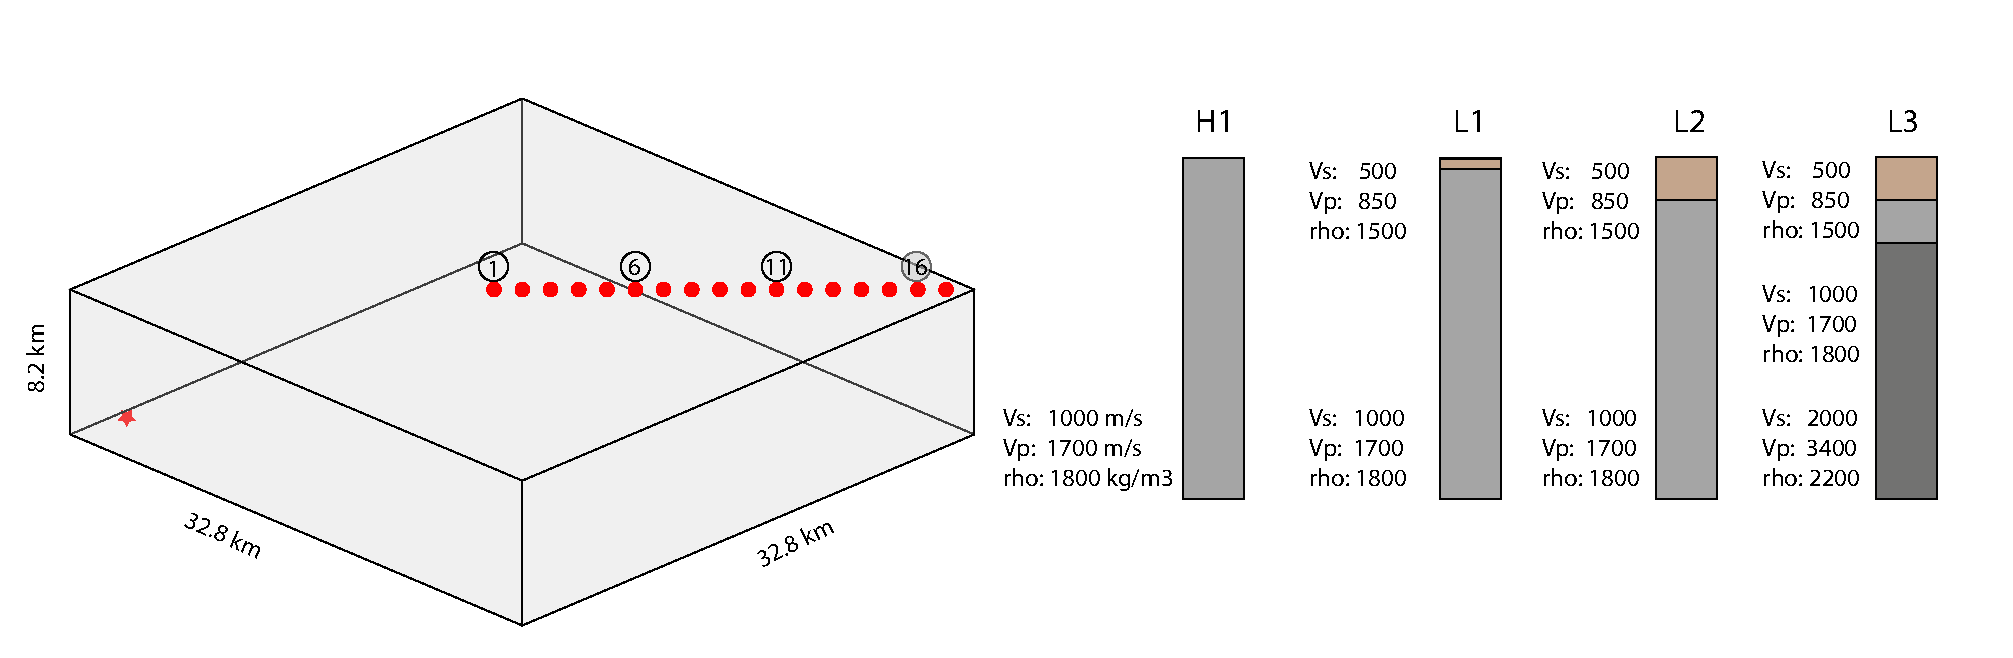
\includegraphics[width=\textwidth]{figures/pdf/3d_domain_scenarios.pdf}
    \caption{Idealized domains to test the proposed method.}
    \label{fig:3d_domain_scenarios}
\end{figure}

Testing of the proposed method is inspired from checker board test idea from inversion studies (add some references). We develop an artificial domain with  known damping parameters, and using the observed data at each stations we search for the initial used parameters. The real heterogeneous region  has greater Los angeles area and also it includes many small basins in different parts. Numerous earthquake recorded in this area and different studies is conducted from different perspective.  Several velocity models are developed and it in an going process \citep[e.g., see][]{small2017scec}. Fig.~\ref{fig:Figure_stations} shows the  heterogeneous domain and stations location. 

 \begin{figure}[ht]
    \centering
    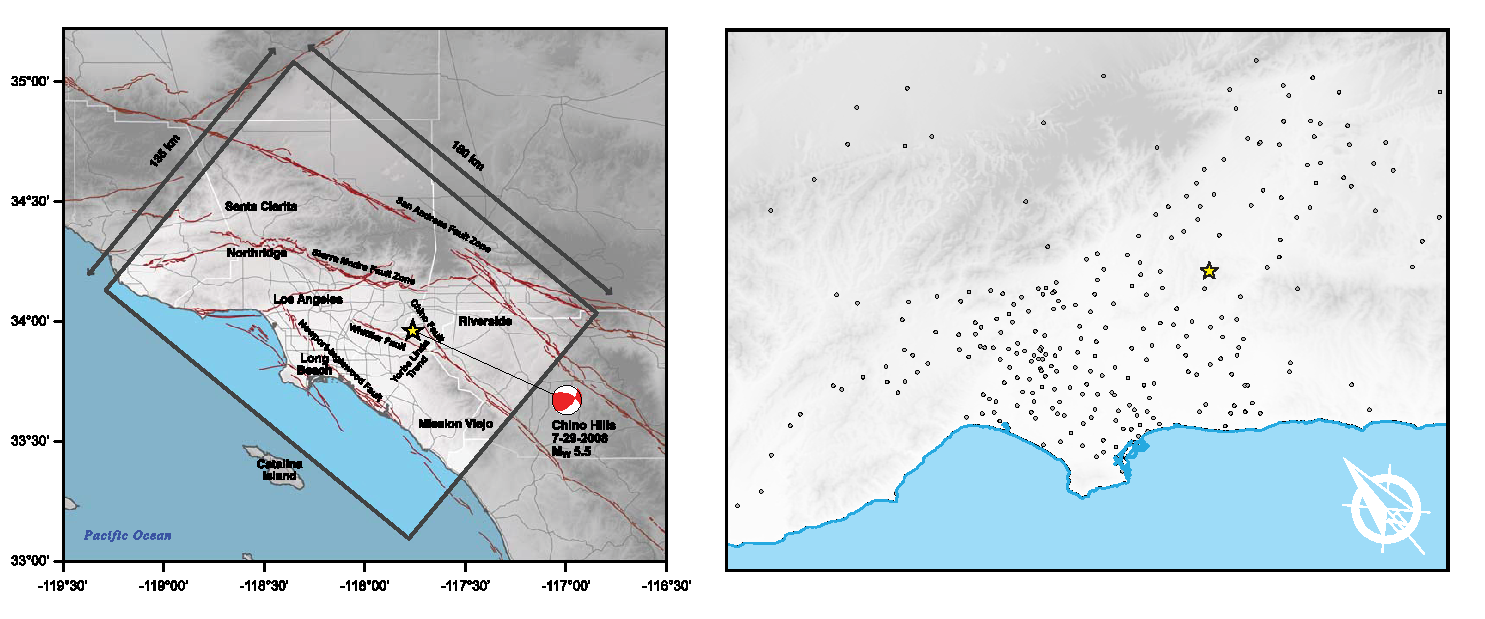
\includegraphics[width=\textwidth]{figures/pdf/Figure_stations.pdf}
    \caption{Processing steps}
    \label{fig:Figure_stations}
\end{figure}


In order to test the methodology with real observational data, we use 2008 $Mw~5.4$  ChinoHills earthquake as an observation platform. Chino Hills earthquake is recored in more than 300 stations. however we only use the strong motion center stations, where in our study simulation box there are 262 stations.  Table.~\ref{tab:event_details}  and Table. ~\ref{tab:sim_param} represent the event and simulation details, respectively. 


\begin{table}[ht]
\centering
\caption{Event details}
\label{tab:event_details}
\renewcommand{\arraystretch}{0.75}
\begin{tabular}{lr}
\\ \hline
Name                                 &   Chino Hills                          \\
Origin Time                        & 29 July 2008 , 11:42 AM             \\
Magnitude                          &  Mw 5.4            \\
Moment                             & 1.566751e+17 Nm             \\
Location/Depth                  &  -117.7613 33.9530 14.7 $Km$    \\
Strike/Dip/Rake                 & 47/51/32                                   \\
3D Crustal Model              & SCEC CVM-S4.26                   \\
Source Model                   & Point Source                                  \\ \hline
\end{tabular}
\end{table}


\begin{table}[ht]
\centering
\caption{Simulation Parameters}
\label{tab:sim_param}
\renewcommand{\arraystretch}{0.75}
\begin{tabular}{lr}
\\ \hline
Domain                              &                              \\
~~Length/Width/Depth       & 180,135,61.875 km \\
~~Southwest corner          & -119.288842, 34.120549             \\
~~Northwest corner           & -118.354016, 35.061096             \\
~~Northeast corner            & -116.846030, 34.025873              \\
~~Southeast corner           & -117.780976, 33.096503               \\
~~Rotation Angle               & 39.9 \\
~~Studied records             & 262 \\
Spatial Resolution              &    \\
~~Maximum frequency     & 1 $Hz$ \\
~~Minimum $V_s$            & 350 m/s \\
~~Points per wavelength   & $9\leq p < 14$\\
~~Minimum size element   & 21.9727 $m$\\
~~Maximum size element   & 351.5625 $m$\\
~~Number of elements       & 157209765 \\
~~Number of nodes            & 180080443 \\
~~Number of dangling nodes & 23681911 \\
Time resolution  & \\
~~Simulation $\Delta$t & 0.002 \\
~~Simulation time & 100 s\\ \hline
\end{tabular}
\end{table}



